%Example of use of Time Domain Astrophysics latex class
\documentclass{tda}

\usepackage[utf8]{inputenc}
%\usepackage[font=footnotesize,labelfont=bf]{caption}
%\captionsetup{width=\columnwidth}
\usepackage{subcaption}

\usepackage{hyperref}
\usepackage[
bibstyle=nature,
giveninits=true,
sorting=none,
natbib=true,
doi=false,
eprint=false,
url=false,
hyperref=true,
date=year
]{biblatex}
\addbibresource{references.bib}
\renewbibmacro{in:}{}

\AtEveryBibitem{%
	\clearfield{note}%
}

\usepackage[font=footnotesize,labelfont=bf]{caption}

\DeclareUnicodeCharacter{2212}{-}
\DeclareUnicodeCharacter{2121}{tel}

%define the page header/title info
\course{Time Domain Astrophysics --- 2020/21 --- Case Study Coursework} %DON'T EDIT ME!

%%%%%%%%%%%%%%%%%%% Change this bit
\topic{Tidal Disruption Events} %DO EDIT ME! Enter the chosen topic, e.g., `Luminous Red Novae'

\begin{document}

\abstract{
Current researches support the possibility that every large galaxy contains a super-massive black hole (SMBH) at its centre. Given that black holes cannot be observed directly, we need to rely upon indirect methods to test inspect their presence. Study of motion of stars in their vicinity near the centres of galaxies like our Milky Way, has helped gather evidence of their presence. On the other hand, study of \emph{tidal disruption events} which occur due to extreme gravitational influence of SMBH on very nearby stars, is another way to probe galactic centres to investigate presence of SMBH. This study focusses on these tidal disruption events, which are transient events that have assisted in understanding numerous phenomena like accretion  disks, dynamics of black holes, properties and evolution of stars near galactic centres, etc.
}

\section{Introduction} \label{introduction}

Motion of stars in central regions of galaxies is influenced by gravitational forces due to other stars as well as black hole at the centre. If a star passes very close to the central black hole, tidal forces on the star may structurally disrupt it. Such an event is called \emph{tidal disruption event} (TDE). These tidal forces are essentially similar in nature to the ones witnessed between earth and moon, that cause tides on earth. 

One condition for tidal disruption to occur is that the star should be close enough to the black hole for tidal forces acting on it to be comparable to its self-gravity \cite{hills_possible_1975}. In that case, 
\[\frac{G m^2}{a^2} \approx \frac{G M^{}_{BH} m}{r_{T}^3} a\]
where \(G\) is universal gravitational constant, \(m\) is the mass of star, \(M^{}_{BH}\) is the mass of black hole, \(a\) is the radius of star and \(r^{}_{T}\) is the minimum pericentre distance between star and black hole at which tidal disruption occurs, called the \emph{tidal radius}. From this, tidal radius can be calculated as \cite{rees_tidal_1988}, 
\begin{equation}
	\Rightarrow r^{}_{T} = \left( \frac{M}{m} \right) ^{\frac{1}{3}} a
	\label{eq:tidal_radius}
\end{equation}

\noindent The Schwarzschild radius of a black hole is given by,
\begin{equation}
	r^{}_{BH} = \frac{2GM^{}_{BH}}{c^2},
	\label{eq:blackhole_radius}
\end{equation}
where \(c\) is the speed of light. From equations \ref{eq:tidal_radius} and \ref{eq:blackhole_radius}, we can compare the dependence of the two distances on black hole mass as,
\begin{equation}
	r^{}_{T} \propto M^{\frac{1}{3}}_{BH}
	\label{eq:tidal_radius_proportionality}
\end{equation}
\begin{equation}
	r^{}_{BH} \propto M^{}_{BH}
	\label{eq:blackhole_radius_proportionality}
\end{equation}
Therefore, beyond a certain mass of black hole, i.e. \(\sim10^8 M_{\odot}\) (\(\sim10^9 M_{\odot}\) upon considering relativistic effects) for a \(1 M_{\odot}\) star, the tidal disruption radius lies inside of black hole event horizon radius as can be seen from figure \ref{fig:rees1990}. In such a case, no observable tidal disruption feature is expected.

\begin{figure} [h]
	\centering
	\begin{minipage} {.45\textwidth}
		\centering
		\captionsetup{width=0.85\linewidth}
		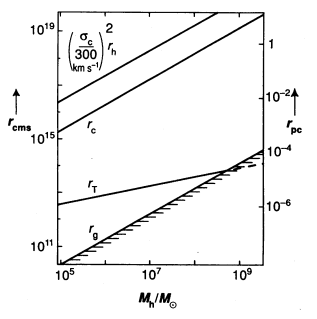
\includegraphics[width=0.9\linewidth]{./images/rees1990.png}
		\caption{TDEs are observationally interesting phenomena only for black holes of mass less than a threshold mass of \(\sim 10^8 M_\odot\) corresponding to \(r^{}_g \approx r^{}_T\). Gravitational radius of black hole is considered as \(r^{}_g = 1.5 \times 10^{13} (M_{BH}/10^8 M_\odot)\)cm. \(r^{}_T\) represents the tidal radius. Adapted from \cite{rees_dead_1990}.}
		\label{fig:rees1990}
	\end{minipage}%
	\begin{minipage} {.45\textwidth}
		\centering
		\captionsetup{width=0.85\linewidth}
		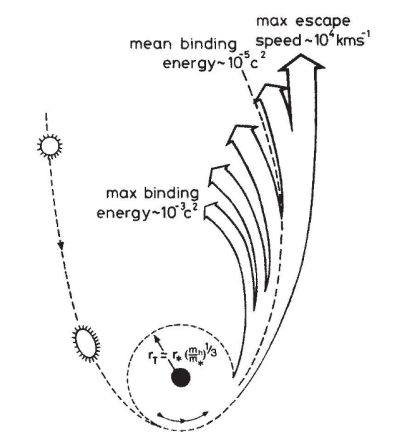
\includegraphics[width=0.9\linewidth]{./images/rees1988.png}
		\caption{A star approaching black hole at pericenter at a distance \(r^{}_T\) gets distorted and tidally disrupted. Nearly half of total mass flies off in unbound hyperbolic orbits while the other half circularizes in bound elliptical orbits. Adapted from \cite{rees_tidal_1988}}
		\label{fig:rees1988}
	\end{minipage}
\end{figure}

For a star moving in parabolic orbit around black hole, after tidal disruption roughly half of stellar matter possesses positive potential energy and flies off unbound, while the other half has negative potential energy and stays in bound elliptical orbits around the black hole as illustrated in figure \ref{fig:rees1988}. This bound matter follows Keplerian orbit of period \(t\) with corresponding energy given by,
\begin{equation}
	E = -\frac{1}{2} \left( \frac{2 \pi G M^{}_{BH}}{t} \right)^\frac{2}{3}
	\label{eq:keplerian_energy}
\end{equation}

This section introduced the basic theoretical aspects of tidal disruption. In section \ref{gen_observations}, the expected and observed rates of these events are compared along with a discussion on observational signatures of TDEs and their underlying causes and variations. Observations using X-rays, UV, optical and radio waves are discussed in section \ref{multiwavelength_astro}, followed by analysis of spectroscopic signatures in section \ref{spectroscopy}. Prospects of observations using astronomical messengers alternate to the electromagnetic waves are discussed in section \ref{multimessenger_astro}. A brief summary concludes this case study in section \ref{summary}.


\section{General Observational Characteristics} \label{gen_observations}

A TDE is a luminous transient event with a usual peak bolometric luminosity \(\sim 10^{41} - 10^{44}\) ergs/s \cite{lodato_multiband_2011, bonnerot_simulating_2020}. The variation of luminosity with time correlates with the mass accretion rate which is numerically equal to the rate of fallback of bound disrupted mass \cite{phinney_manifestations_1989}. This rate can be obtained using equation \ref{eq:keplerian_energy} as,
\begin{equation}
	L \propto \frac{dM}{dt} = \frac{dM}{dE} \frac{dE}{dt} = k \frac{dM}{dE} t^{-5/3},
	\label{eq:tde_luminosity_time}
\end{equation}
where, \[k=\frac{\left({2 \pi G M^{}_{BH}}\right)^{\frac{2}{3}}}{3}\]

\noindent In the case of complete disruption of star in a close encounter, considered in \cite{evans_tidal_1989, lodato_stellar_2009}, the energy distribution through the mass is uniform (i.e. \(\frac{dM}{dE} = \) constant). Therefore, in that case, \(L \propto \dot{M} \propto t^{-5/3}\). In reality, this relation holds true for bolometric luminosities only at late times \cite{lodato_stellar_2009, lodato_multiband_2011} as seen in figures \ref{fig:lodato2009a} and \ref{fig:lodato2009b} and is taken to be the characteristic observational signature of a TDE, while at early times, this rate correlates strongly with the type of disrupted star and its properties \cite{lodato_stellar_2009, lodato_recent_2015, guillochon_hydrodynamical_2013}. This correlation holds till the process of \emph{circularization}, i.e. the disk formation occurs. Later, at some point accretion of circularized debris begins, the emission from which follows the \(t^{-5/3}\) law and is therefore a subject of observational interest in order to characterize TDE candidates \cite{piran_disk_2015}.

Recently, very few TDEs have been observed to exhibit another observable feature -- relativistic jets \cite{lodato_recent_2015}. Some models have linked jet formation to strong magnetic fields and black hole spin \cite{dai_unified_2018}. Jets are not observed generally, but in cases where they have been observed, they have provided insights into the conditions around black holes.

Theoretical models expect TDEs to occur at a rate of \(\sim 10^{-4}\) events per year per galaxy \cite{magorrian_rates_1999}. However, observations from the past decades provide an estimate roughly an order of magnitude lower, at \(\sim 10^{-5}\) events per year per galaxy \cite{stone_rates_2016}, possibly due to selection effects and observational limitations. A rate of \((2.2–17.0) \times 10^{−5}\) events per year per galaxy with \(90\%\) confidence interval is calculated using \textit{ASAS-SN} observations \cite{holoien_six_2016}. However, when contribution from faint TDEs along with bias towards bright TDEs is considered, this value rises upto \(1.7_{-1.3}^{+2.7} \times 10^{-4}\) per year per galaxy \cite{hung_sifting_2018}. 

\begin{figure}
	\begin{subfigure} {.33\linewidth}
		\centering
		\captionsetup{width=.85\linewidth}
		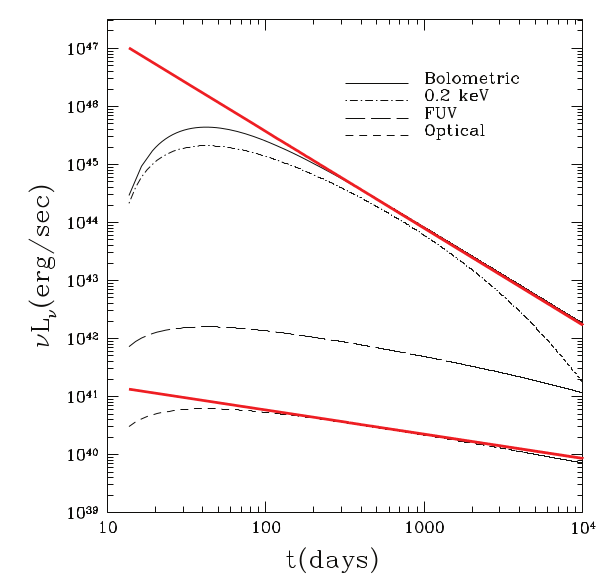
\includegraphics[width=\textwidth]{./images/lodato_rossi2011.png}
		\caption{Light curves for the disc emission from the disruption of a solar-type star by a \(10^6 M_\odot\) black hole. The two red lines mark the simple power laws
expected for the bolometric luminosity (\(\propto t^{-5/3}\)) and for the monochromatic
luminosity in the optical/UV (\(\propto t^{-5/12}\)). Adapted from \cite{lodato_multiband_2011}.}
	\label{fig:lodatorossi2011}
	\end{subfigure}
	\begin{subfigure} {.33\linewidth}
		\centering
		\captionsetup{width=.85\linewidth}
		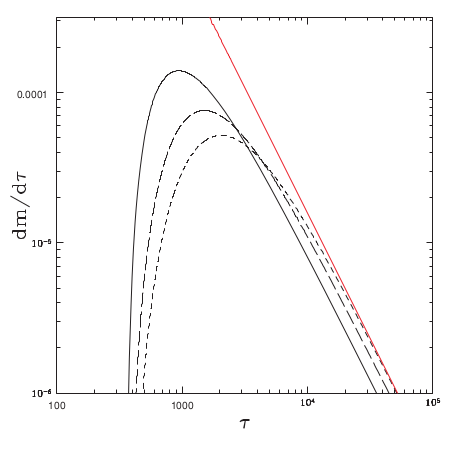
\includegraphics[width=\textwidth]{./images/lodato2009a.png}
		\caption{Evolution of accretion rate for star with different properties and stellar parameters. The red line indicates \(t^{-5/3}\) power law for reference. Adapted from \cite{lodato_stellar_2009}}
		\label{fig:lodato2009a}
	\end{subfigure}
	\begin{subfigure} {.33\linewidth}
		\centering
		\captionsetup{width=.85\linewidth}
		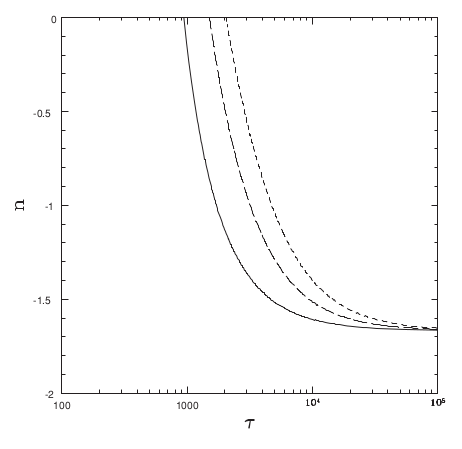
\includegraphics[width=\textwidth]{./images/lodato2009b.png}
		\caption{Time evolution of power law index, corresponding to different stellar parameters in figure \ref{fig:lodato2009a}. The value of \(n=-5/3\) is approached at late times in all cases. Adapted from \cite{lodato_stellar_2009}.}
		\label{fig:lodato2009b}
	\end{subfigure}
	\caption{Deviation of TDE luminosities from the \(t^{-5/3}\) law}
\end{figure}

\section{Multi-wavelength Observations} \label{multiwavelength_astro}


\subsection{X-rays} \label{multiwave:xrays}

The emission from a TDE peaks in the soft X-ray -- UV part of the electromagnetic spectrum. As a consequence X-ray observatories like \textit{ROSAT}, \textit{Chandra}, \textit{Swift}, \textit{NuSTAR} and \textit{XMM Newton} have been used extensively to study TDEs since 1990s.

RXJ1242.6-1119 and TDE in the galaxy NGC 5905 have been extensively studied over long term and can be considered as representative cases of general X-ray TDE observations. X-ray luminosity increased over the initial few days, with peak in soft X-ray band, which decreased over the next months and years by factor of few thousands as the peak shifted towards the hard X-ray band. The X-ray luminosity decline followed the \(t^{-5/3}\) law \cite{komossa_tidal_2015} as seen in figure \ref{fig:xray_luminosity}.

Subsequent searches of X-ray observatories databases, especially \textit{ROSAT} and \textit{XMM Newton} have revealed TDEs in optically quiescent nearby galaxies \cite[see references in][]{komossa_tidal_2015} with X-ray luminosities ranging from \(\sim 10^{42}\) ergs/s to more than \(\sim 10^{44}\) ergs/s. Accordingly, less that \(10\%\) of stellar mass was needed to power the emissions in most cases. Also, most of the computed black hole masses are of the order of \(10^6 - 10^8 M_{\odot}\). The spectral energy distribution is peaked at high temperatures (\(\approx 10^5\)K).

From X-ray observations of TDE in SDSSJ120136.02+300305.5 using \textit{Swift}, the first supermassive binary black hole candidate was identified, which showed characteristic gaps in observed lightcurve predicted by theoretical models \cite{liu_miliparsec_2014}.


\subsection{Ultraviolet} \label{multiwave:uv}

The \textit{Galaxy Evolution Explorer}, or the \textit{GALEX} satellite has been the only significant sky survey so far for TDE observations in UV band of electromagnetic spectrum \cite{van_velzen_optical-ultraviolet_2020}. It assisted in the long term multi-wavelength study of TDEs \cite{gezari_ultraviolet_2006}. All TDE candidates follow the \(t^{-5/3}\) law and have simple blackbody spectra \cite{nicholas_chamberlain_stone_tidal_2013}. The computed size of emitting blackbodies turns out to be extremely large. This is due to reprocessed emission from large outer shell consistent with theoretical predictions \cite{ulmer_flares_1999}. Spectral energy distribution is peaked at low temperatures (\(\approx 10^4\)K).

\subsection{Optical} \label{multiwave:optical}

Although the optical emissions from a TDE are not as prominent as X-ray or UV emissions, several optical surveys, like \textit{PTF}, \textit{Pan-STARRS}, \textit{SDSS} and \textit{ASAS-SN} have studied as well as discovered transient TDE flares. Many of these events did not have detectable X-ray counterparts due to low temperatures. With recent and upcoming highly efficient high cadence observatories for observing transients like the \textit{Vera C. Rubin Observatory (LSST)} and \textit{eROSITA}, significant study of TDEs in optical waveband can be expected in the near future \cite{strubbe_optical_2009}. By comparing figures \ref{fig:xray_luminosity} and \ref{fig:optical UV_luminosity}, it can be seen that early time development of TDE flares is more densely samples in optical/UV bands than for X-ray bands. This makes study of correlation of luminosity variation on stellar properties in early times is possible using optical/UV data \cite{gezari_tidal_2013}. 

Theoretically, optical luminosity variation with time is expected to follow the relation \(L \propto t^{-5/12}\) \cite{lodato_multiband_2011}. However, unexpectedly, many of the optical observations roughly follow the \(t^{-5/3}\) law instead. One reason for this might be significant reprocessing of emissions, but the topic is still under active research.

\begin{figure} 
	\begin{minipage} {.5 \textwidth}
		\captionsetup{width=.85\linewidth}
		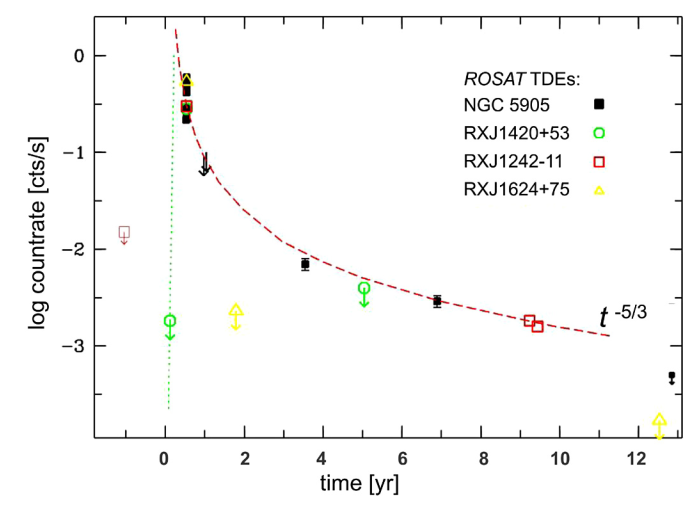
\includegraphics[width=0.9\linewidth]{./images/komossa2015.png}
		\caption{Joint X-ray lightcurve of five ROSAT TDEs, all shifted to the same peak time. The dashed line represents the \(t^{-5/3}\) curve for reference. Adapted from \cite{komossa_tidal_2015}}
		\label{fig:xray_luminosity}
	\end{minipage}%
	\begin{minipage} {.5 \textwidth}
		\captionsetup{width=.85\linewidth}
		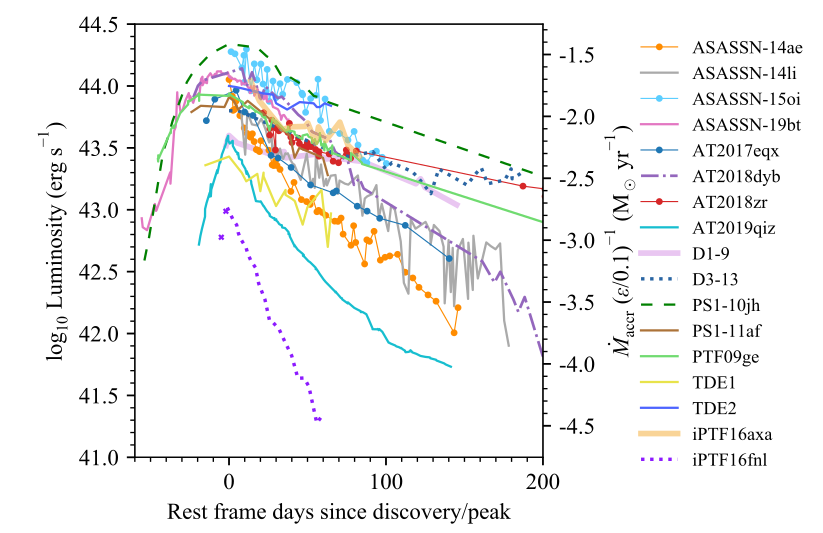
\includegraphics[width=\linewidth]{./images/vanvelzen2020.png}
		\caption{Lightcurves of UV/optical TDEs. The integrated optical-ultraviolet luminosity is shown as inferred
from spectral energy distribution fitting. The mass accretion rate on the right hand side is normalized to an efficiency \(\epsilon\) of 0.1. Adapted from \cite{van_velzen_optical-ultraviolet_2020}}
		\label{fig:optical UV_luminosity}
	\end{minipage}
\end{figure}

\subsection{Radio} \label{multiwave:radio}

Detections of radio emissions are mostly associated with outflow of matter, producing shocks in the circumnuclear medium \cite{bonnerot_first_2021}. Most TDEs do not launch powerful radio jets, however there have been exceptions \cite{komossa_tidal_2015}, with lightcurves of nine confirmed radio jets from TDEs shown in figure \ref{fig:radio_luminosity}. \textit{VLA} has been used to study radio emissions from X-ray emitting TDE candidates. Recently, a possibility has been suggested that radio emission from TDEs might correspond to changes in accretion states \cite{horesh_delayed_2021}.

\begin{figure} [h]
	\centering
	\captionsetup{width=.85\linewidth}
	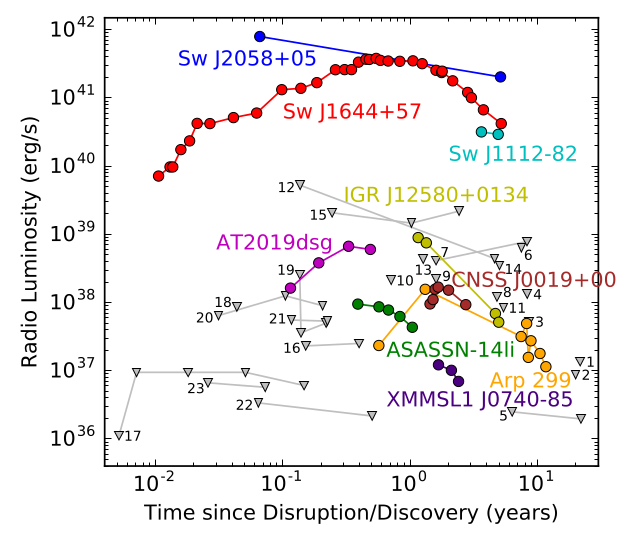
\includegraphics[width=.35\linewidth]{./images/alexander2020.png}
	\caption{Nine published TDE radio observations, each at single frequency, are shown using coloured circles. Additional 23 events \cite{alexander_radio_2020} with published upper limits are represented with grey triangles. Adapted from \cite{alexander_radio_2020}.}
	\label{fig:radio_luminosity}
\end{figure}

\newpage
\section{Spectroscopy} \label{spectroscopy}

\begin{figure}
	\centering
	\captionsetup{width=.85\linewidth}
	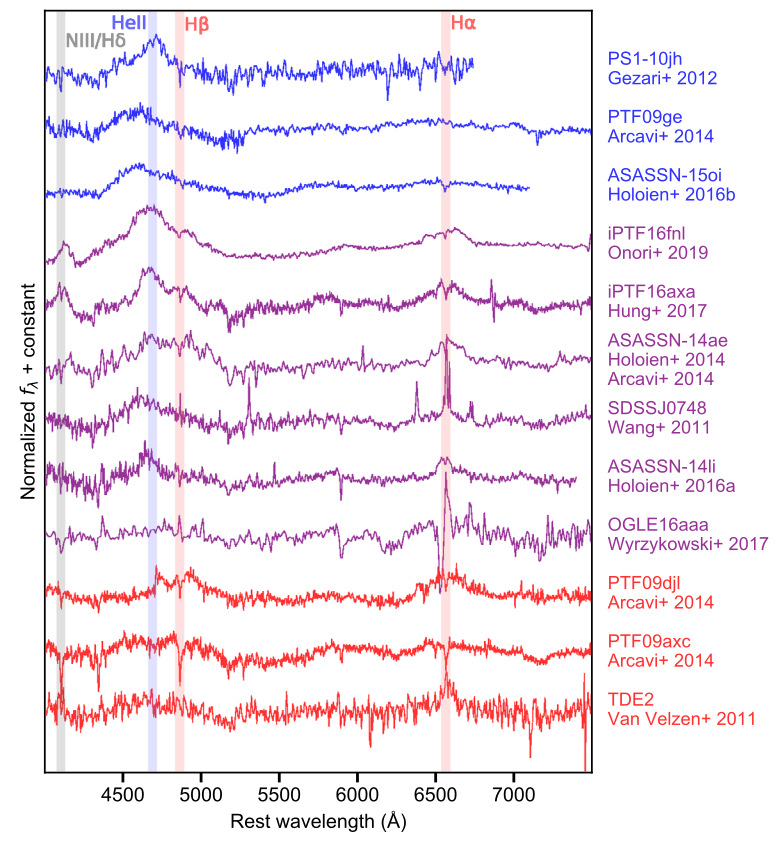
\includegraphics[width=.5\linewidth]{./images/arcavi2014.png}
	\caption{Continuum-subtracted optical spectra of optically-discovered TDEs \cite{arcavi_continuum_2014}. Events in blue are dominated by
a broad He II feature with no signatures of H\(\alpha\) or H\(\beta\). Events in purple
are characterized by the presence of both broad He II and H\(\alpha\), with possible broad H\(\beta\) seen in some events.Events in red are H-dominated. Additional N III features (perhaps blended with
H\(\delta\)) are seen for some events in the “H+He” class. Adapted from \cite{van_velzen_optical-ultraviolet_2020}.}
	\label{fig:spectrographs}
\end{figure}

As emission from TDE flare passes through the intervening matter, the X-ray--UV continuum get transformed to emission spectrum. Spectra of all TDEs show bright broad emission from He and/or H, which probably arise from the accreting matter \cite{guillochon_hydrodynamical_2013, komossa_tidal_2015} and fade on timescales of several months to years \cite{komossa_tidal_2015, wang_transient_2011}, . Some spectra in gas rich environments show transient super-strong iron coronal lines of upto Fe\(^{13+}\) ionization states \cite{wang_transient_2011}. These high ionization lines fade over time and become undetectable after a few years. The broad H and He lines also fade over time while the lower ionization lines increase in strength relatively. A comparison of different spectroscopic signatures of TDEs can be seen in figure \ref{fig:spectrographs}. Emission from unbound stellar debris is expected to be very faint. Velocities of materials involved in TDEs are also inferred spectroscopically to understand the morphology of the event.

Spectroscopy can be used to distinguish TDEs from other types of transients. Spectra corresponding to higher temperatures than those of typical supernovae help differentiate TDEs from supernovae. Active galactic nuclei, which are recurring and have different magnitude of outbursts, also have features in their spectra which are very distinct from those of TDEs \cite{arcavi_continuum_2014}.


\section{Multi-messenger Observations} \label{multimessenger_astro}

TDEs are targets for multi-messenger astronomy with interesting observable aspects of cosmic rays, neutrinos and gravitational waves.

Origin and evolution of cosmic ray particles in TDEs are inspected in \cite{zhang_high-energy_2017}. Ultra-high energy cosmic rays find it hard to survive in luminous and powerful TDE jets. Main sequence stars and carbon-oxygen white dwarfs do not produce the observed cosmic ray spectrum and hence cannot be the source of TDE cosmic rays. While the oxygen-neon-magnesium white dwarfs can successfully produce the spectrum, they might be too rare to be the true sources of these cosmic rays. Therefore, a lot potential lies in theoretical and observational understanding of cosmic ray phenomena from TDEs.

Neutrino observations can be used to probe several aspects of TDEs, especially the jets. Neutrino observatories with their large field of view can detect TDEs at higher rates if their electromagnetic counterparts can be detected \cite{wang_probing_2011}. Consequently, part of unaccounted flux obtained at large neutrino observatories may be attributed to TDEs \cite{lunardini_high_2017}. High energy cosmic ray protons can produce neutrinos after interacting with the X-ray photons which are present in large quantities in TDE flares. Efficient production of neutrinos with lack of cosmic rays is expected for luminous TDEs, while high energy cosmic rays with poor production of neutrinos is expected for TDEs with low luminosities \cite{zhang_high-energy_2017}. 

Supermassive black hole binaries can be discovered via TDEs, like the one mentioned in section \ref{multiwave:xrays}. Such binaries will produce gravitational waves upon merger \cite{komossa_tidal_2015}. Also, tidal disruption of a white dwarf by intermediate mass black hole is expected to be a source of detectable gravitational waves. Time variation in quadrupole moment of star-black hole system causes emission of marginally detectable low frequency gravitational waves as the star travels past the orbital pericenter on its parabolic orbit \cite{kobayashi_gravitational_2004, nicholas_chamberlain_stone_tidal_2013}.  

\section{Summary} \label{summary}

\begin{figure} [h]
	\centering
	\captionsetup{width=.85\linewidth}
	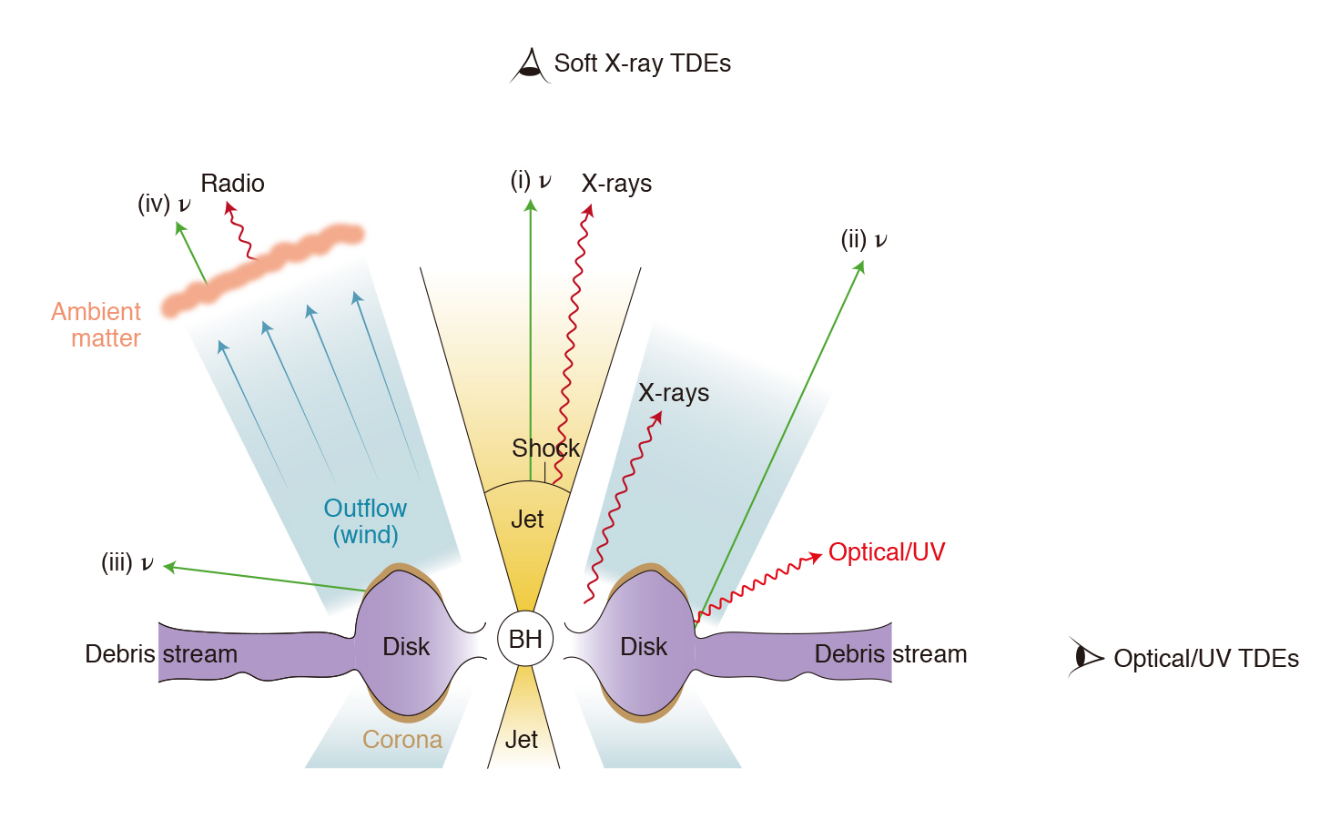
\includegraphics[width=.7\linewidth, height=.3\linewidth]{./images/hayasaki2021.png}
	\caption{An illustration of the disk-outflow-jet system formed after tidal disruption of a star. Depending on the viewing angle, the
waveband of observable thermal emission from TDEs changes from soft X-rays to the UV/optical. Four different sources of neutrinos are also indicated by \(\nu\). Adapted from \cite{hayasaki_neutrinos_2021}}
	\label{fig:em_neutrino_sources}
\end{figure}

TDEs form an important class of luminous transient events and constitute an actively growing research domain representing various scientific interests. From observational perspective, they can be studied over a wide range of wavelengths in the electromagnetic spectrum and using all types of astronomical messengers, i.e. electromagnetic waves, cosmic rays, neutrinos and gravitational waves. Sources of different electromagnetic waves and neutrinos are illustrated in figure \ref{fig:em_neutrino_sources}. While X-rays, UV and optical wavelengths find their origins in accretion disk, jet and debris, the radio waves originate when shocks interact with circumnuclear matter. Interest in TDEs is no longer limited to observations of tidal disruption in black hole-star systems, but now extends to disruptions in planet-satellite systems as well as star-planet systems, etc.

Theoretically, the early works done in the 1970s and 1980s established the basic formalism and successfully account for many of the important observations. Today, large scale hydrodynamical simulations have revealed much more informations of the intricate details of tidal disruption phenomena. However, there still remain many unanswered questions as some subtle aspects of existing theory are being challenged and probed by comparison with observed data. Taking spins of black holes and relativistic aspects of processes into consideration further complicate the numerical studies. Initial lightcurves for TDEs vary substantially for different systems, but at later times, roughly follow the \(t^{-5/3}\) luminosity law, often (unexpectedly) at optical and UV wavelengths also.

Studying TDEs help us understand the physics of accretion disks and of extreme environments around black holes. In near future, as capability to collect more and better data increases, TDEs are expected to assist in analysis of the demographics of black holes. Distributions of mass and spin along with other statistical properties of massive black holes can also be explored using TDEs. A subset of these events which possess jets have intrigued many researchers in recent times, as their study helps in investigating the formation and evolution of jets, which in turn aids understanding of other jetted astrophysical phenomena.

\clearpage
\printbibliography

\end{document}
